\setmodule{9}

%BEGIN_FOLD % ====>>_____ Занятие 1 _____<<====
\begin{class}[number=1]
	\begin{listofex}
		\item Занятие 1
	\end{listofex}
\end{class}
%END_FOLD

%BEGIN_FOLD % ====>>_____ Занятие 2 _____<<====
\begin{class}[number=2]
	\begin{listofex}
		\item Занятие 2
	\end{listofex}
\end{class}
%END_FOLD

%BEGIN_FOLD % ====>>_ Домашняя работа 1 _<<====
\begin{homework}[number=1]
	\begin{listofex}
		\item Решите уравнения:
		\begin{tasks}(2)
			\task \( (x-1)^4-2(x-1)^2-3=0 \)
			\task \( (x+4)^4-6(x+4)^2-6=0 \)
		\end{tasks}
		\item Собственная скорость лодки \( 8,5 \) км/ч, а скорость течения \( 3,5 \) км/ч. Расстояние между пристанями \( 15 \) км. Сколько времени затратит лодка на путь между пристанями туда и обратно?
		\item Два велосипедиста выехали из двух сёл одновременно навстречу друг другу и встретились через \( 1,6 \) ч. Скорость первого \( 10 \) км/ч, а второго --- \( 12 \) км/ч. Найдите расстояние между сёлами?
	\end{listofex}
\end{homework}
%END_FOLD

%BEGIN_FOLD % ====>>_____ Занятие 3 _____<<====
\begin{class}[number=3]
	\begin{listofex}
		\item Занятие 3 
	\end{listofex}
\end{class}
%END_FOLD

%BEGIN_FOLD % ====>>_____ Занятие 4 _____<<====
\begin{class}[number=4]
	\begin{listofex}
		\item Занятие 4
	\end{listofex}
\end{class}
%END_FOLD

%BEGIN_FOLD % ====>>_ Домашняя работа 2 _<<====
\begin{homework}[number=2]
	\begin{listofex}
		\item 
		\begin{minipage}[t]{\bodywidth}
			Дано: \( \angle A = \angle B \), \( CO = 4 \), \( DO = 6 \), \( AO = 5  \). Найти:\begin{tasks}(2)
				\task \( OB \)
				\task \( AC : BD \) 
				\task \( S_{AOC} : S_{BOD} \)
			\end{tasks}
		\end{minipage}
		\hspace{0.02\linewidth}
		\begin{minipage}[t]{\picwidth}
			% TODO: \usepackage{graphicx} required
			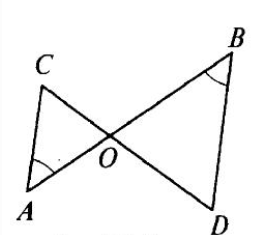
\includegraphics[align=t, width=\linewidth]{../../../../../exercises/lists/pics/G81M9H1-1}
		\end{minipage}
		\item На сторонах \( AB \) и \( BC \) треугольника \( ABC \) отмечены точки \( K \) и \( E \) так, что \( AK=KB \), \( BE=CE \), \( KE=6 \) см. Найдите сторону \( AC \).
		\item  Прямая, параллельная основанию треугольника, делит его на треугольник и трапецию, площади которых относятся как \( 4:5 \). Периметр образовавшегося треугольника равен \( 20 \) см. Найдите периметр.
		\item Человек ростом \( 1,7 \) м стоит на расстоянии \( 8 \) метров от столба, на котором висит фонарь. Тень человека равна \( 4 \) метрам. На какой высоте в метрах расположен фонарь?
		\item Отрезки \( KE \) и \( MN \) пересекаются в точке \( O \), так что отрезок \( KM \) параллелен отрезку \( NE \). Докажите, что треугольники \( KMO \) и \( NEO \) подобны. Найдите \( KM \), если \( ON=6 \) см, \( MO=12 \) см, \( NE=18 \) см.
	\end{listofex}
\end{homework}
%END_FOLD

%BEGIN_FOLD % ====>>_____ Занятие 5 _____<<====
\begin{class}[number=5]
	\begin{listofex}
		\item Занятие 5
	\end{listofex}
\end{class}
%END_FOLD

%BEGIN_FOLD % ====>>_____ Занятие 6 _____<<====
\begin{class}[number=6]
	\begin{listofex}
		\item Занятие 6
	\end{listofex}
\end{class}
%END_FOLD

%BEGIN_FOLD % ====>>_ Домашняя работа 3 _<<====
\begin{homework}[number=3]
	\begin{listofex}
		\item Домашняя работа 3
	\end{listofex}
\end{homework}
%END_FOLD

%BEGIN_FOLD % ====>>_____ Занятие 7 _____<<====
\begin{class}[number=7]
	\title{Подготовка к проверочной}
	\begin{listofex}
		\item Занятие 7
	\end{listofex}
\end{class}
%END_FOLD

=%BEGIN_FOLD % ====>>_ Проверочная работа _<<====
\begin{exam}
	\begin{listofex}
		\item Проверочная
	\end{listofex}
\end{exam}
%END_FOLD